\documentclass[conference]{IEEEtran}
\IEEEoverridecommandlockouts

\usepackage{cite}
\usepackage{amsmath,amssymb,amsfonts}
\usepackage{algorithmic}
\usepackage{algorithm}
\usepackage{graphicx}
\usepackage{textcomp}
\usepackage{xcolor}
\usepackage{booktabs}
\usepackage{multirow}
\usepackage{url}

\graphicspath{{../../benchmarks/plots/}{../../benchmarks/plots/mpi/}}

\begin{document}

\title{Adaptive Heterogeneous Parallel Framework for\\High-Resolution Urban Flood Simulation}

\author{
\IEEEauthorblockN{Arushi Vaidya}
\IEEEauthorblockA{\textit{Department of Computer Science and Engineering}\\
\textit{RV College of Engineering}\\
Bengaluru, India\\
USN: 1RV23CS049}
\and
\IEEEauthorblockN{Aryan Gupta}
\IEEEauthorblockA{\textit{Department of Computer Science and Engineering}\\
\textit{RV College of Engineering}\\
Bengaluru, India\\
USN: 1RV23CS051}
}

\maketitle

\begin{abstract}
High-resolution urban flood simulation is computationally expensive because it
combines large spatial domains, fine grid resolution and thousands of time
steps of the two-dimensional shallow-water equations (SWE). This paper presents
an adaptive heterogeneous parallel framework that couples a conservative
finite-volume SWE solver with adaptive mesh refinement (AMR) and four parallel
programming models: OpenMP for shared memory, MPI for distributed memory, and
CUDA and OpenACC for accelerators. All backends share one numerical
formulation (hydrostatic reconstruction, Rusanov fluxes, a positivity-preserving
flux limiter, rainfall, infiltration and implicit Manning friction), so their
results can be compared bit for bit. On a synthetic urban district with
buildings, streets and a river surge, a $128\times128$ OpenMP run reproduces the
serial reference exactly (maximum depth difference $0$\,m), conserves mass to
$10^{-10}$\,m$^3$, and predicts the flood extent of a $2\times$ finer reference
with an intersection-over-union (IoU) of 95.3\% and a mean relative depth
error of 4.4\%. On a dam-break case, AMR matches a $4\times$ finer uniform
solution (IoU 100\%, relative error 0.10\%) while using $4.9\times$ fewer cells.
MPI reaches a parallel efficiency of 94\% on two ranks for a $512\times512$
grid. A 42-test regression suite and an interactive web laboratory accompany
the framework.
\end{abstract}

\begin{IEEEkeywords}
urban flood modelling, shallow-water equations, finite-volume method, adaptive
mesh refinement, OpenMP, MPI, CUDA, OpenACC, heterogeneous computing
\end{IEEEkeywords}

%=====================================================================
\section{Introduction}
%=====================================================================
Pluvial and fluvial flooding are among the most damaging natural hazards in
rapidly urbanising regions. Physically based flood models solve the
depth-averaged shallow-water equations over a digital elevation model (DEM),
but urban features such as buildings, kerbs and streets only appear at metre
resolution. A city-scale domain at that resolution has millions of cells, and
the explicit time step allowed by the Courant--Friedrichs--Lewy (CFL)
condition shrinks as the cells get smaller. The cost therefore grows roughly
with the third power of the refinement factor.

Two complementary strategies reduce this cost: \emph{parallelism}, which
spreads the work over cores, nodes and accelerators, and \emph{adaptivity},
which spends resolution only where the flow is active. Recent work has
explored GPU, multi-GPU and dynamically adaptive flood models
\cite{saleem2024,rong2024,wang2024,chen2025,dong2025,chowdhury2025}, but most
systems commit to one programming model and use uniform effort across the
domain.

This work makes the following contributions:
\begin{enumerate}
\item A single conservative finite-volume SWE formulation implemented in five
backends (serial, OpenMP, MPI, CUDA, OpenACC), with the accelerator kernels
written once as structure-of-arrays device functions shared by CUDA and OpenACC.
\item A block-structured AMR solver with flux-conserving coarse/fine interfaces
and optional dynamic load balancing across MPI ranks.
\item An evaluation methodology that reports runtime, speedup, efficiency,
mass conservation, and flood-extent accuracy (IoU and depth-error
distribution) against a higher-resolution uniform reference.
\item An open, test-driven implementation with 42 automated regression tests
and an interactive laboratory that runs the real solver and visualises it.
\end{enumerate}

%=====================================================================
\section{Related Work}
%=====================================================================
Saleem and Norman \cite{saleem2024} built a scalable shallow-water solver with
MPI and OpenACC on GPUs and reported strong scaling for large flood domains.
Rong \emph{et al.} \cite{rong2024} used non-uniform grids on GPUs to resolve
buildings and roads efficiently. Wang \emph{et al.} \cite{wang2024} introduced
local time stepping on GPUs for domains with heterogeneous flow conditions.
Chen \emph{et al.} \cite{chen2025} combined multi-GPU execution with AMR and
dynamic load balancing. Dong \emph{et al.} \cite{dong2025} developed a
multi-GPU finite-volume model for large-scale flood simulation, and Chowdhury
and Kesserwani \cite{chowdhury2025} extended LISFLOOD-FP with GPU acceleration
and on-the-fly resolution adaptivity.

The numerical building blocks used here are classical: the Rusanov
(local Lax--Friedrichs) flux \cite{rusanov1961}, the hydrostatic reconstruction
of Audusse \emph{et al.} \cite{audusse2004} for well-balanced wet/dry
treatment, and finite-volume methods for free-surface flow \cite{toro2001}.
Block-structured AMR follows Berger and Oliger \cite{berger1984} and the
conservative coarse/fine flux correction of Berger and Colella
\cite{berger1989}. The parallel models are OpenMP \cite{dagum1998}, MPI
\cite{gropp2014}, CUDA \cite{nickolls2008} and OpenACC \cite{openacc}.

The remaining gaps are uniform computational effort in low-activity regions,
high memory cost, limited integration of adaptivity and load balancing in
heterogeneous setups, and communication overhead at scale. This framework
targets the first three directly and measures the fourth.

%=====================================================================
\section{Mathematical Model and Numerical Method}
%=====================================================================
\subsection{Governing Equations}
The two-dimensional shallow-water equations in conservative form are
\begin{equation}
\frac{\partial \mathbf{U}}{\partial t} + \frac{\partial \mathbf{F}(\mathbf{U})}{\partial x}
+ \frac{\partial \mathbf{G}(\mathbf{U})}{\partial y} = \mathbf{S}(\mathbf{U}),
\label{eq:swe}
\end{equation}
\begin{equation}
\mathbf{U}=\begin{bmatrix} h\\ hu\\ hv\end{bmatrix},\;
\mathbf{F}=\begin{bmatrix} hu\\ hu^2+\tfrac12 g h^2\\ huv\end{bmatrix},\;
\mathbf{G}=\begin{bmatrix} hv\\ huv\\ hv^2+\tfrac12 g h^2\end{bmatrix},
\end{equation}
where $h$ is water depth, $(u,v)$ the depth-averaged velocity and $g$
gravitational acceleration. The source term contains bed slope, rainfall $R(t)$,
infiltration $I$ and Manning friction with roughness $n$:
\begin{equation}
\mathbf{S}=\begin{bmatrix} R-I\\ -gh\,\partial_x z - \dfrac{g n^2 u\lvert\mathbf{u}\rvert}{h^{1/3}}\\[4pt]
-gh\,\partial_y z - \dfrac{g n^2 v\lvert\mathbf{u}\rvert}{h^{1/3}}\end{bmatrix}.
\end{equation}

\subsection{Finite-Volume Discretisation}
On a Cartesian grid with spacing $\Delta x,\Delta y$, cell averages are
updated by
\begin{equation}
\mathbf{U}_i^{n+1} = \mathbf{U}_i^{n} - \frac{\Delta t}{\lvert\Omega_i\rvert}
\sum_{f\in\partial\Omega_i} \phi_f\,\mathbf{F}^{*}_f\,\ell_f + \Delta t\,\mathbf{S}_i,
\end{equation}
where $\ell_f$ is the face length and $\phi_f\in[0,1]$ is a positivity limiter.

\textbf{Hydrostatic reconstruction.} At each face the bed is taken as
$z_f=\max(z_L,z_R)$ and the reconstructed depths are
$h_{L,R}^{*}=\max(0,\,h_{L,R}+z_{L,R}-z_f)$ \cite{audusse2004}. This keeps a
lake at rest exactly at rest and lets building cells, whose bed is raised by
6--22\,m, act as impermeable obstacles without special treatment.

\textbf{Rusanov flux.} With reconstructed states $\mathbf{U}_L^*,\mathbf{U}_R^*$,
\begin{equation}
\mathbf{F}^{*} = \tfrac12\big(\mathbf{F}(\mathbf{U}_L^*)+\mathbf{F}(\mathbf{U}_R^*)\big)
- \tfrac12 s_{\max}\big(\mathbf{U}_R^*-\mathbf{U}_L^*\big),
\end{equation}
with $s_{\max}=\max\big(\lvert u_L\rvert+\sqrt{g h_L^*},\,\lvert u_R\rvert+\sqrt{g h_R^*}\big)$.
The pressure difference between $h$ and $h^*$ is added to the momentum flux
on each side to balance the bed-slope source.

\textbf{Positivity.} Each face's mass flux is assigned to its donor cell. If a
cell's total outgoing volume $Q_i\Delta t$ exceeds its stored volume
$h_i\lvert\Omega_i\rvert$, all its outgoing fluxes are scaled by
$\phi_i = h_i\lvert\Omega_i\rvert/(Q_i\Delta t)$. Depth therefore never becomes
negative and the update stays conservative.

\textbf{Time step.} The explicit step satisfies
\begin{equation}
\Delta t = \min\!\left(\frac{C}{\max_i\!\left(\frac{\lvert u_i\rvert+\sqrt{gh_i}}{\Delta x}+\frac{\lvert v_i\rvert+\sqrt{gh_i}}{\Delta y}\right)},\;\Delta t_{\max}\right),
\end{equation}
with $C=0.4$. It is also cut so that steps land exactly on changes in the
rainfall hyetograph.

\textbf{Friction and wet/dry.} Manning friction is applied semi-implicitly,
$\mathbf{q}^{n+1} = \mathbf{q}^{*}/(1+\Delta t\, g n^2 \lvert\mathbf{u}\rvert h^{-4/3})$,
which is unconditionally stable for shallow water. Cells with
$h\le 10^{-6}$\,m are treated as dry and their momentum is set to zero.

\textbf{Boundaries.} Closed walls reflect the normal momentum. Outflow
boundaries copy the interior state but forbid inflow. All boundary volumes are
accumulated so that the global balance
$V_0 + V_{\text{rain}} - V_{\text{out}} - V_{\text{inf}} - V_{\text{stored}}$
can be reported as a mass residual.

%=====================================================================
\section{Framework Architecture}
%=====================================================================
The framework follows the five-stage pipeline in Fig.~\ref{fig:pipeline}:
(1) input and preprocessing of terrain, land use, rainfall and boundary
conditions; (2) domain decomposition; (3) the parallel solver; (4) adaptive
spatial resolution; and (5) time stepping, output and evaluation.

\begin{figure}[t]
\centering
\setlength{\fboxsep}{4pt}
\fbox{\parbox{0.92\columnwidth}{\centering\small
\textbf{1. Input \& preprocessing} (DEM, buildings, rainfall, BCs)\\[2pt]
$\downarrow$\\[2pt]
\textbf{2. Domain decomposition} (MPI 2-D blocks / OpenMP chunks / GPU threads)\\[2pt]
$\downarrow$\\[2pt]
\textbf{3. Parallel FV solver} (Serial $|$ OpenMP $|$ MPI $|$ CUDA $|$ OpenACC)\\[2pt]
$\updownarrow$\\[2pt]
\textbf{4. Adaptive resolution} (activity indicator, refine/coarsen, load balance)\\[2pt]
$\downarrow$\\[2pt]
\textbf{5. Output \& evaluation} (depth, momentum, mass balance, IoU, speedup)}}
\caption{Processing pipeline of the framework.}
\label{fig:pipeline}
\end{figure}

\subsection{Shared-Memory Backend (OpenMP)}
The serial and OpenMP backends share one source routine. Every per-cell and
per-face loop (CFL reduction, $x$- and $y$-face fluxes, donor bookkeeping,
limiter, flux accumulation and cell update) is annotated with
\texttt{\#pragma omp parallel for} with a static schedule and
\texttt{collapse(2)} on the face loops. The CFL step uses a \texttt{max}
reduction. Face fluxes go into separate arrays and each cell gathers from its
four faces, so there are no write conflicts and no atomics. This is why OpenMP
results are bitwise identical to the serial reference.

\subsection{Distributed-Memory Backend (MPI)}
The global grid is split into a 2-D Cartesian block layout from
\texttt{MPI\_Dims\_create} and \texttt{MPI\_Cart\_create}. Rank 0 scatters
packed cell states; each rank keeps a one-cell halo and exchanges it with its
four neighbours every step. The time step is agreed with an
\texttt{MPI\_Allreduce(MIN)}, and the volume budgets are reduced at the end.
Timings are split into computation, communication and synchronisation.

\subsection{Accelerator Backends (CUDA and OpenACC)}
The accelerator kernels are written once as structure-of-arrays (SoA) device
functions (\texttt{FlatKernels.hpp}) marked \texttt{\_\_host\_\_ \_\_device\_\_}
under CUDA and \texttt{\#pragma acc routine seq} under OpenACC. The CUDA
backend keeps $h,hu,hv$ and the bed on the device for the whole run and
launches one thread per face or cell for the flux, limiter and update kernels.
It uses Thrust reductions for the CFL rate, boundary outflow, infiltration and
validity checks, so only scalars cross the PCIe bus each step. The OpenACC
backend expresses the same loop nest with \texttt{parallel loop} regions
inside one \texttt{acc data} region.

Without an OpenACC compiler the directives are ignored and the same loop nest
runs on the host. This is how the shared kernels are regression-tested on any
machine: on all seven built-in scenarios the host execution matches the
serial solver with a maximum state difference of exactly zero
(Table~\ref{tab:validation}). The CUDA and OpenACC backends are built only
when CMake detects \texttt{nvcc} or an OpenACC-capable compiler; otherwise
they report themselves unavailable instead of silently falling back.

\subsection{Adaptive Mesh Refinement}
The adaptive solver uses a block-structured hierarchy of $8\times8$ patches with
refinement ratio 2 and up to two levels (cells $4\times$ finer than the base).
Every two steps a flood-activity indicator built from water depth, velocity
and their gradients is evaluated per patch. Patches above a refinement threshold
(0.10) are refined and patches below a coarsening threshold (0.05) are
coarsened. At coarse/fine interfaces the coarse flux is replaced by the sum of
fine-face fluxes (refluxing \cite{berger1989}), so mass is conserved exactly
across levels. The adaptive backends are serial, OpenMP and MPI. In MPI,
patches can be migrated between ranks when the workload imbalance
(max/mean) exceeds 1.2, with a cooldown of 10 steps between rebalances.

%=====================================================================
\section{Experimental Setup}
%=====================================================================
\subsection{Platform}
All measurements were taken on an Apple M2 system-on-chip (8 CPU cores:
4 performance and 4 efficiency) running macOS, with Apple Clang 16,
Homebrew \texttt{libomp} and Open MPI. The machine has no NVIDIA GPU, so CUDA
and OpenACC were verified for correctness through the shared host kernels but
not timed on a GPU. Runtimes are solver wall time, excluding I/O.

\subsection{Scenarios}
\begin{itemize}
\item \textbf{Urban district}: a synthetic city defined in normalised
coordinates, so it is identical at every resolution. It has a meandering river
with a 3.4\,m surge in its upstream reach, a 9$\times$9 street grid lowered
0.18\,m below the kerbs, building footprints 6--22\,m tall, parks, a storm of
120\,mm/h for 60\,s then 40\,mm/h, Manning $n=0.035$, and outflow boundaries.
Cells are 5\,m; the simulated time is 120\,s.
\item \textbf{Dam break}: a 1\,m column of water released over a flat bed,
used for the AMR study.
\item Benchmark cases: flat basin, slope, rain-and-drain, wet/dry front and
lake at rest, used by the regression suite.
\end{itemize}

\subsection{Metrics}
Speedup is $S_p = T_{\text{serial}}/T_p$ and efficiency is $E_p = S_p/p$.
Flood-extent accuracy is measured against a uniform serial solution at
$k\times$ the resolution, block-averaged back to the model grid. A cell counts
as flooded if $h>0.05$\,m. With predicted set $P$ and reference set $R$,
\begin{equation}
\text{IoU} = \frac{\lvert P\cap R\rvert}{\lvert P\cup R\rvert}.
\end{equation}
Depth errors $\lvert h-h_{\text{ref}}\rvert$ are collected over $P\cup R$, and
the relative error is the mean absolute error divided by the mean reference
depth over the same cells.

%=====================================================================
\section{Results}
%=====================================================================
\subsection{Correctness and Conservation}
Table~\ref{tab:validation} summarises the verification evidence. All 42
CTest regression tests pass. They cover the serial solver, OpenMP/serial
consistency, MPI consistency on 1--6 ranks across six scenarios, the adaptive
grid, adaptive serial/OpenMP/MPI solvers, load balancing, capability
reporting and the shared accelerator kernels.

\begin{table}[t]
\caption{Verification Summary}
\label{tab:validation}
\centering
\begin{tabular}{@{}lr@{}}
\toprule
Check & Result \\
\midrule
CTest regression suite & 42/42 passed \\
OpenMP vs.\ serial, urban $128^2$ (max $\lvert\Delta h\rvert$) & 0\,m \\
Accelerator kernels vs.\ serial, 7 scenarios & 0 (bitwise) \\
Mass residual, urban $128^2$ & $\sim\!10^{-10}$\,m$^3$ \\
Accelerator mass residual, 7 scenarios & $\le 4\times10^{-11}$\,m$^3$ \\
AMR coarse/fine interface residual & 0 \\
\bottomrule
\end{tabular}
\end{table}

\subsection{Flood-Extent Accuracy}
Table~\ref{tab:accuracy} reports accuracy against high-resolution references.
In the urban district the $128\times128$ model (5\,m cells) reproduces the flood
extent of the $256\times256$ reference (2.5\,m cells) with IoU 95.3\%,
precision 98.6\% and recall 96.5\%. Most disagreement is a slight
under-prediction of the flood edge in narrow streets, which the finer grid
resolves. The depth-error distribution is strongly right-skewed: mean
0.026\,m, standard deviation 0.031\,m, RMSE 0.041\,m, giving a mean relative
error of 4.4\%. On the coarser $96\times96$ grid the IoU drops to 93.1\% and
the relative error rises to 5.6\%, which is the expected convergence trend.

\begin{table}[t]
\caption{Accuracy Against High-Resolution Uniform References}
\label{tab:accuracy}
\centering
\begin{tabular}{@{}lccc@{}}
\toprule
Case & IoU & Rel.\ err. & RMSE \\
\midrule
Urban $96^2$ vs.\ $192^2$ & 93.1\% & 5.6\% & 0.049\,m \\
Urban $128^2$ vs.\ $256^2$ & 95.3\% & 4.4\% & 0.041\,m \\
Dam break AMR (L2) vs.\ $4\times$ uniform & 100\% & 0.10\% & 0.003\,m \\
\bottomrule
\end{tabular}
\end{table}

\subsection{Adaptive Resolution}
For a $64\times64$ dam break with two refinement levels, the adaptive solution
used 13{,}312 active leaf cells, compared with 65{,}536 for a uniform grid at
the finest resolution: a $4.9\times$ reduction. Its flood extent matched the
$4\times$ uniform reference exactly (IoU 100\%) with a mean relative depth
error of 0.10\%. Refinement followed the moving bore, and the rest of the
domain stayed coarse.

A limitation appeared in the rain-driven urban scenario. Rainfall wets every
cell, and the building walls create steep gradients everywhere, so the
activity indicator refined the whole domain ($16\times$ the base cell count)
and adaptivity gave no benefit. Activity-based AMR therefore pays off for
localised events (dam breaks, river surges, flash floods) rather than
domain-wide pluvial flooding. Pluvial flooding needs indicators that ignore
thin sheet flow and static obstacles.

\subsection{Parallel Performance}
Table~\ref{tab:perf} lists measured speedups. OpenMP gives
$1.7$--$2.2\times$ on four threads. It is limited by memory bandwidth (the
update streams several arrays per cell with little arithmetic) and by the
heterogeneous M2 cores: the four efficiency cores slow the static schedule when
more than four threads are used. MPI reaches $1.88\times$ on two ranks
(94\% efficiency) for a $512\times512$ flat basin. Communication is under 1\%
of runtime at that size because the halo grows with the perimeter while the
work grows with the area.

\begin{table}[t]
\caption{Measured Parallel Performance (Apple M2)}
\label{tab:perf}
\centering
\begin{tabular}{@{}llcc@{}}
\toprule
Case & Backend & Speedup & Efficiency \\
\midrule
Dam break $128^2$ & OpenMP, 4 thr. & 1.76$\times$ & 44\% \\
Flat basin $1024^2$ & OpenMP, 4 thr. & 2.05$\times$ & 51\% \\
Urban $128^2$ & OpenMP, 4 thr. & 1.7--2.2$\times$ & 42--55\% \\
Flat basin $512^2$ & MPI, 2 ranks & 1.88$\times$ & 94\% \\
\bottomrule
\end{tabular}
\end{table}

\begin{figure}[t]
\centering
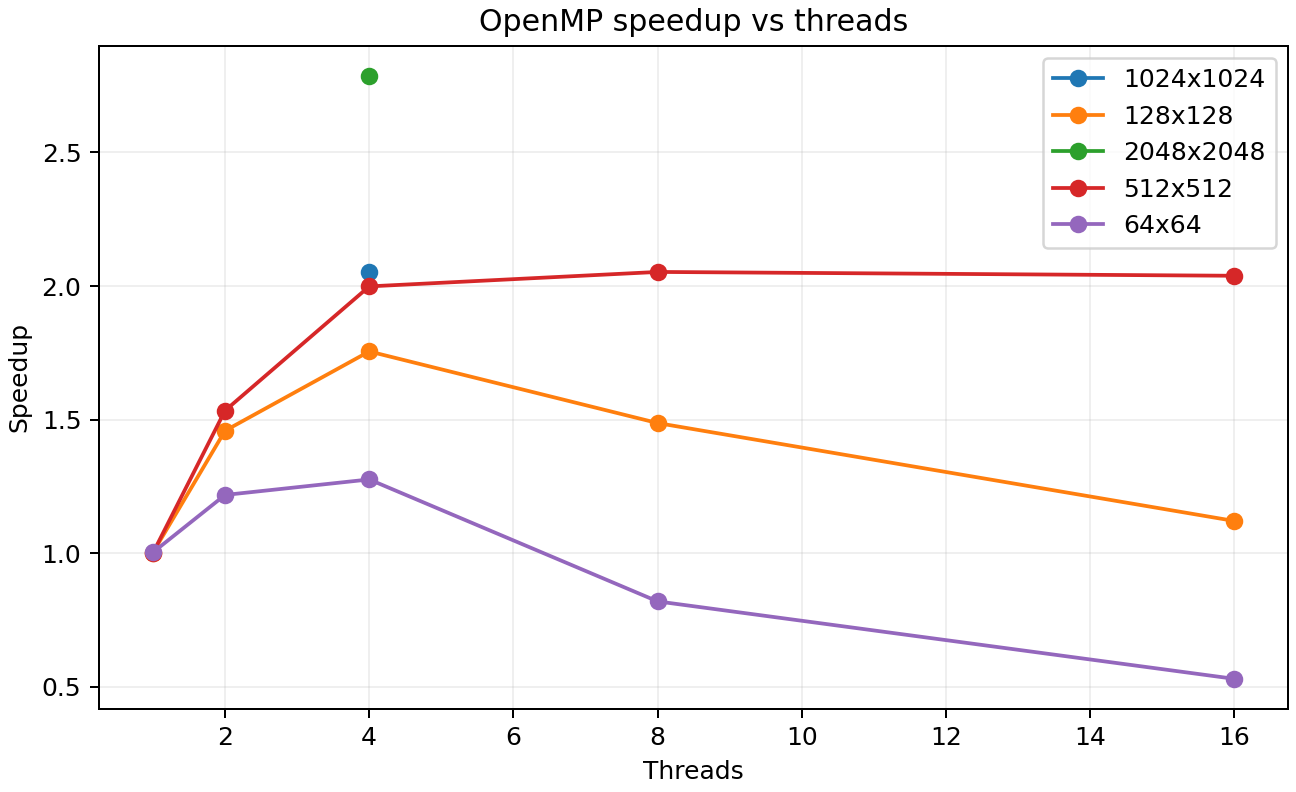
\includegraphics[width=0.95\columnwidth]{openmp_speedup.png}
\caption{OpenMP speedup against thread count (measured).}
\label{fig:omp}
\end{figure}

\begin{figure}[t]
\centering
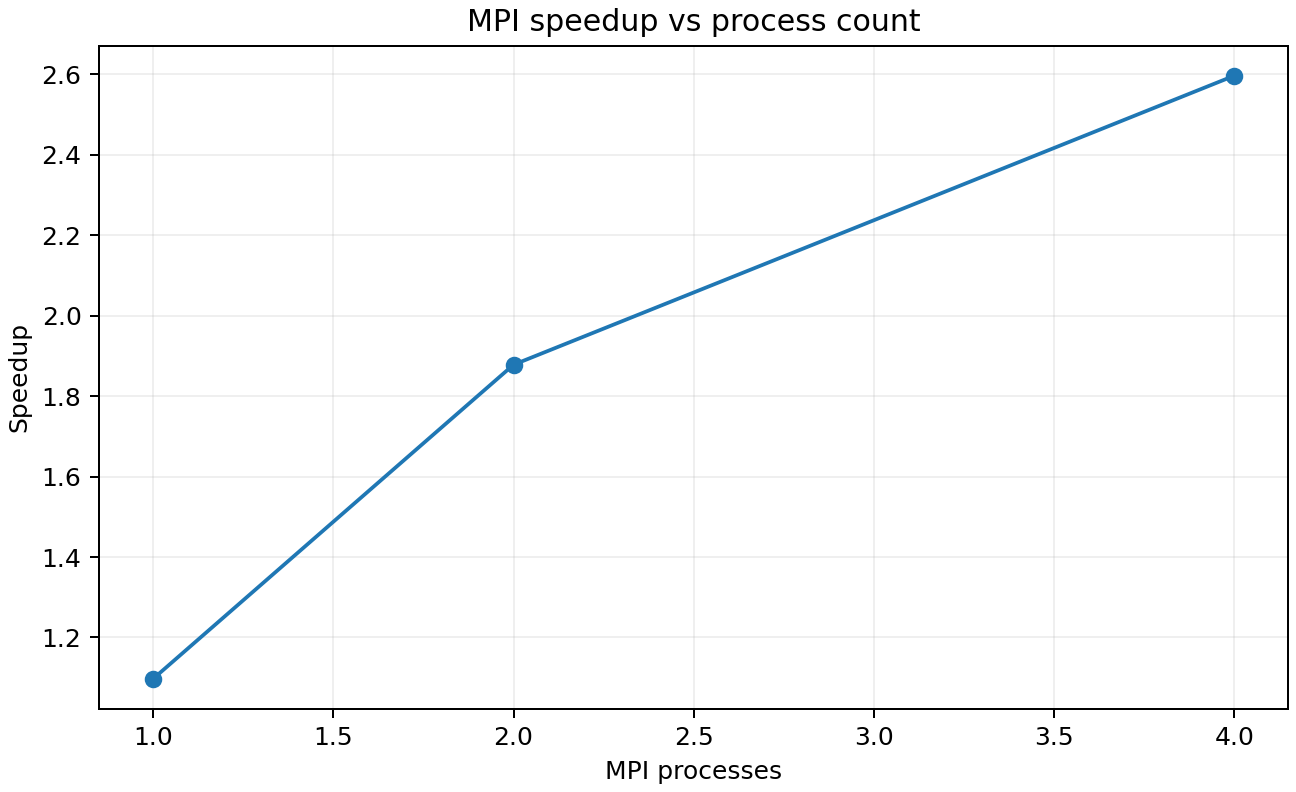
\includegraphics[width=0.95\columnwidth]{mpi_speedup.png}
\caption{MPI speedup against process count (measured).}
\label{fig:mpi}
\end{figure}

%=====================================================================
\section{Interactive Simulation Laboratory}
%=====================================================================
A local web laboratory (\texttt{scripts/ui.py}) launches the C++ solver with a
chosen scenario, backend, thread or rank count, grid size, storm and physics
parameters (rain intensity and duration, Manning $n$, infiltration, boundary
type, river surge, reservoir level and breach width). Every run is
automatically compared with a serial reference and a $2\times$ (uniform) or
$2^{L}\times$ (adaptive) resolution reference. The laboratory replays the
solver's own time-lapse frames as an aerial view: land use, rooftops with sun
shadows, depth-shaded water, and flow tracers integrated through the computed
velocity field. It also shows the AMR patch hierarchy, the MPI block
decomposition, the live pipeline stage, and the outcome metrics (IoU, speedup,
throughput and the error histogram). Every displayed number comes from a run;
nothing is interpolated or estimated.

%=====================================================================
\section{Discussion and Limitations}
%=====================================================================
The scenarios are synthetic. The accuracy figures measure convergence towards
a finer numerical solution, not agreement with observed floods; calibration
against surveyed flood marks is future work. CUDA and OpenACC were verified
for correctness but not benchmarked on GPU hardware. The scheme is
first-order in space and time, so a MUSCL reconstruction with a two-stage
Runge--Kutta integrator would cut numerical diffusion at the same resolution.
Finally, the activity indicator should be extended for pluvial events, and
GPU-resident AMR is a natural next step.

%=====================================================================
\section{Conclusion}
%=====================================================================
We presented an adaptive heterogeneous parallel framework for high-resolution
urban flood simulation. It puts one conservative, well-balanced
finite-volume SWE formulation behind OpenMP, MPI, CUDA and OpenACC backends
and couples it with flux-conserving AMR and dynamic load balancing.
Parallel runs reproduce the serial reference bit for bit and conserve mass to
round-off. The urban model predicts the flood extent of a $2\times$ finer
reference with 95.3\% IoU and 4.4\% relative depth error, and AMR delivers
fine-grid accuracy with $4.9\times$ fewer cells for localised floods. The
measured speedups show where the shared-memory and distributed backends help.
They also show the main open problem: making adaptivity pay off for
domain-wide pluvial flooding.

\section*{Acknowledgment}
The authors thank the Department of Computer Science and Engineering, RV
College of Engineering, for guidance in the Parallel Architectures and GPU
Programming (PAGP) laboratory.

\begin{thebibliography}{00}
\bibitem{saleem2024} S.~Saleem and M.~R.~Norman, ``A scalable shallow-water solver for flood modelling using MPI, OpenACC and GPUs,'' \textit{Environmental Modelling \& Software}, vol.~181, Art.~no.~106364, 2024.
\bibitem{rong2024} Y.~Rong, X.~Liu, and Z.~Wang, ``GPU-accelerated urban flood modelling with nonuniform grids,'' \textit{Journal of Hydrology}, vol.~643, Art.~no.~131972, 2024.
\bibitem{wang2024} X.~Wang, H.~Li, and Q.~Zhang, ``A GPU-accelerated shallow-water model with local time stepping for efficient flood simulation,'' \textit{Advances in Water Resources}, vol.~186, Art.~no.~104724, 2024.
\bibitem{chen2025} J.~Chen, Z.~Li, and Y.~Zhao, ``Multi-GPU urban flood simulation with adaptive mesh refinement and load balancing,'' \textit{Computers \& Fluids}, vol.~281, Art.~no.~106354, 2025.
\bibitem{dong2025} W.~Dong, L.~Guo, and H.~Sun, ``A multi-GPU finite-volume shallow-water model for large-scale flood simulation,'' \textit{Water Resources Research}, vol.~61, no.~4, Art.~no.~e2024WR036821, 2025.
\bibitem{chowdhury2025} A.~Chowdhury and G.~Kesserwani, ``LISFLOOD-FP 8.2: GPU-accelerated flood modelling with on-the-fly dynamic resolution adaptivity,'' \textit{Environmental Modelling \& Software}, vol.~188, Art.~no.~106488, 2025.
\bibitem{rusanov1961} V.~V.~Rusanov, ``The calculation of the interaction of non-stationary shock waves and obstacles,'' \textit{USSR Computational Mathematics and Mathematical Physics}, vol.~1, no.~2, pp.~304--320, 1962.
\bibitem{audusse2004} E.~Audusse, F.~Bouchut, M.-O.~Bristeau, R.~Klein, and B.~Perthame, ``A fast and stable well-balanced scheme with hydrostatic reconstruction for shallow water flows,'' \textit{SIAM Journal on Scientific Computing}, vol.~25, no.~6, pp.~2050--2065, 2004.
\bibitem{toro2001} E.~F.~Toro, \textit{Shock-Capturing Methods for Free-Surface Shallow Flows}. Chichester, U.K.: Wiley, 2001.
\bibitem{berger1984} M.~J.~Berger and J.~Oliger, ``Adaptive mesh refinement for hyperbolic partial differential equations,'' \textit{Journal of Computational Physics}, vol.~53, no.~3, pp.~484--512, 1984.
\bibitem{berger1989} M.~J.~Berger and P.~Colella, ``Local adaptive mesh refinement for shock hydrodynamics,'' \textit{Journal of Computational Physics}, vol.~82, no.~1, pp.~64--84, 1989.
\bibitem{dagum1998} L.~Dagum and R.~Menon, ``OpenMP: An industry standard API for shared-memory programming,'' \textit{IEEE Computational Science and Engineering}, vol.~5, no.~1, pp.~46--55, 1998.
\bibitem{gropp2014} W.~Gropp, E.~Lusk, and A.~Skjellum, \textit{Using MPI: Portable Parallel Programming with the Message-Passing Interface}, 3rd~ed. Cambridge, MA, USA: MIT Press, 2014.
\bibitem{nickolls2008} J.~Nickolls, I.~Buck, M.~Garland, and K.~Skadron, ``Scalable parallel programming with CUDA,'' \textit{ACM Queue}, vol.~6, no.~2, pp.~40--53, 2008.
\bibitem{openacc} OpenACC-Standard.org, ``The OpenACC Application Programming Interface, Version 3.3,'' 2022. [Online]. Available: \url{https://www.openacc.org}
\end{thebibliography}

\end{document}
